\section{Pipeline de Voxelización} % (fold)
\label{sec:pipeline_de_voxelizacion}
El algoritmo de voxelización de escenas es implementado en una clase que hereda de la clase Renderer. En el método Render, residen la lógica por el lado de la CPU de voxelización, sombreado de vóxeles, \emph{mipmapping} para vóxeles anisótropos e iluminación global de vóxeles. En esta sección se describe en detalle solo el proceso de voxelización y su arquitectura.
\subsection{Arquitectura}

La arquitectura de nuestro proceso de voxelización describe un pipeline, donde la entrada es geometría, materiales, texturas y matrices de proyección y la salida es una serie de volúmenes de vóxeles los cuales describen una discretización de esta geometría.

El algoritmo de voxelización se ejecuta entre el \emph{geometry shader} y el \emph{fragment shader}. En el \emph{geometry shader} se proyecta y traslada los vértices de cada triángulo para generar un triángulo expandido. La rasterización conservativa de cada triángulo es tarea de ambos shaders. El \emph{fragment shader} primeramente descarta fragmentos excedentes de la expansión del triángulo en el \emph{geometry shader} para formar un polígono delimitante. La voxelización de geometría estática y dinámica se realiza sobre este mismo pipeline, el \emph{fragment shader} debe garantizar que los vóxeles estáticos no sean sobrescritos durante la voxelización dinámica, finalmente se realiza una operación de promedio sobre todos los atributos de cada fragmento que forma parte del espacio que envuelve un vóxel, este valor es almacenado luego en cada vóxel por atributo. En la Figura \ref{fig:voxel_pipeline_impl} se puede observar la composición de esta arquitectura.
\begin{figure}[H]
    \centering
    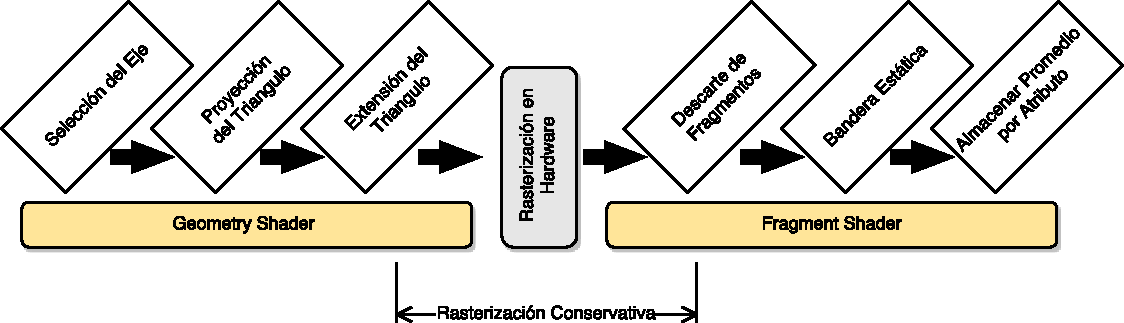
\includegraphics[width=\linewidth]{media/voxel_pipeline_cropped.pdf}
    \caption{Descripción gráfica del pipeline de voxelización.}
    \label{fig:voxel_pipeline_impl}
\end{figure}

\subsection{Voxelización Conservativa} % (fold)
\label{sub:voxelization_impl}
Nuestra implementación utiliza una representación simplificada de la escena en vóxeles, esta representación es generada de forma conservativa por tanto si existe algún triángulo dentro del espacio de un vóxel se generara un vóxel por más pequeño que sea este triángulo.
 
\subsubsection{Matrices de Proyección por Eje}

Como se explicó en la sección \ref{sub:voxelizacion_conservativa} cada triángulo debe ser proyectado sobre un eje direccional. El primer paso a realizar es definir estas matrices de proyección. Estas están definidas por una \ac{AABB} uniforme. En nuestra implementación se toma la \ac{AABB} que envuelve toda la escena por simplicidad. En el Código \ref{UpdateProjectionMatrices} se encuentra el algoritmo de la función que realiza esto. Este método se invoca cada vez que se carga una escena o cuando se cambia la resolución de la representación en vóxeles.

La \ac{AABB} puede estar definida de dos formas: por un punto que indica el centro de la caja y un vector extensión que indica la longitud media de la caja en cada eje a partir del centro o por un punto mínimo y un punto máximo. 
\\
\begin{lstlisting}[caption={Creación de matrices de proyección ortogonal por cada eje direccional}, label=UpdateProjectionMatrices]
void VoxelizerRenderer::UpdateProjectionMatrices(const BoundingBox &sceneBox)
{
    // longitud del aabb en cada eje
    auto axisSize = sceneBox.Extent() * 2.0f;
    // centro del aabb
    auto &center = sceneBox.Center();
    // tamaño de la cuadrícula de vóxeles
    volumeGridSize = glm::max(axisSize.x, glm::max(axisSize.y, axisSize.z));
    // tamaño de un vóxel en la cuadrícula
    voxelSize = volumeGridSize / volumeDimension;
    auto halfSize = volumeGridSize / 2.0f;
    // proyección ortogonal
    auto projection = glm::ortho(-halfSize, halfSize, -halfSize, halfSize, 0.0f, volumeGridSize);
    // matrices de vista por cada eje
    viewProjectionMatrix[0] = lookAt(center + glm::vec3(halfSize, 0.0f, 0.0f), center, glm::vec3(0.0f, 1.0f, 0.0f));
    viewProjectionMatrix[1] = lookAt(center + glm::vec3(0.0f, halfSize, 0.0f), center, glm::vec3(0.0f, 0.0f, -1.0f));
    viewProjectionMatrix[2] = lookAt(center + glm::vec3(0.0f, 0.0f, halfSize), center, glm::vec3(0.0f, 1.0f, 0.0f));
    // multiplicación de ambas matrices para obtener la matriz de proyección para los triángulos
    for (auto &matrix : viewProjectionMatrix) { matrix = projection * matrix; }
}
\end{lstlisting}

En el Código \ref{UpdateProjectionMatrices} se observa que primero se obtiene la longitud total en cada eje que define la \ac{AABB} que envuelve la escena. Luego en la misma función se actualizan dos variables: \emph{volumeGridSize} que indica el tamaño de la cuadrícula tridimensional de vóxeles en espacio de mundo y \emph{voxelSize} que indica el tamaño de cada vóxel dentro de esta cuadrícula. 

El tronco de proyección es un cubo uniforme por tanto se utiliza la mayor longitud según cada eje. Esto asegura que desde cualquier eje direccional la proyección abarca toda la escena. De esta longitud se extrae la matriz de proyección ortogonal. Luego se configura cada matriz de vista por cada eje direccional. Finalmente se almacena la multiplicación de ambas matrices.

Una vez obtenidas las matrices de proyección el algoritmo procede a voxelizar la escena. El proceso de voxelización estática y dinámica utilizan el mismo programa de sombreado o \emph{shader}, la diferencia reside sobre cual geometría es enviada al pipeline de rasterización y durante el \emph{fragment shader} si se lee o se escribe sobre una textura que indica las posiciones de vóxeles estáticos.

\subsubsection{Selección del Eje Dominante}
Para maximizar el área de voxelización y generar la mayor cantidad de fragmentos posibles cada triángulo es proyectado sobre uno de los ejes direccionales (ver Figura \ref{fig:axis_selection}). Este eje se escoge según el vector normal definido por el plano formado por los tres vértices del triángulo. Este proceso se realiza en el \emph{geometry shader}. En el \emph{geometry shader} se pueden realizar operaciones sobre los vértices generados por el procesador de vértices o \emph{vertex shader}. Esto es de particular interés para el proceso de voxelización conservativa ya que como fue explicado anteriormente cada vértice de cada triángulo necesita ser expandido.
\\
\begin{lstlisting}[caption={Selección del eje dominante para la proyección ortogonal.}, label=CalculateAxis]
int CalculateAxis()
{
    // normal del plano formado por vertices del triángulo
    vec3 p1 = gl_in[1].gl_Position.xyz - gl_in[0].gl_Position.xyz;
    vec3 p2 = gl_in[2].gl_Position.xyz - gl_in[0].gl_Position.xyz;
    vec3 faceNormal = cross(p1, p2);

    // valor por eje direccional
    float nDX = abs(faceNormal.x);
    float nDY = abs(faceNormal.y);
    float nDZ = abs(faceNormal.z);

    // índice para la matriz de proyección
    if( nDX > nDY && nDX > nDZ )
    {
        return 0;
    }
    else if( nDY > nDX && nDY > nDZ  )
    {
        return 1;
    }
    else
    {
        return 2;
    }
}
\end{lstlisting}

En el Código \ref{CalculateAxis} primero se obtiene el vector normal del triángulo. El arreglo \emph{gl\_in} contiene información de todos los vértices generados por el vertex shader. Para la aplicación esto es forzado a solo triángulos, por tanto la longitud de gl\_in siempre es tres. Luego según el peso en cada eje del vector normal del plano formado por el triángulo se escoge un eje direccional. Esto se retorna como un número entero. Este número indica cuál de las matrices de proyección generadas en la sección anterior va ser utilizada para proyectar cada vértice del triángulo.

\begin{figure}[H]
	\centering
	\begin{subfigure}[t]{.49\linewidth}
		\centering
		\captionsetup{justification=centering}
		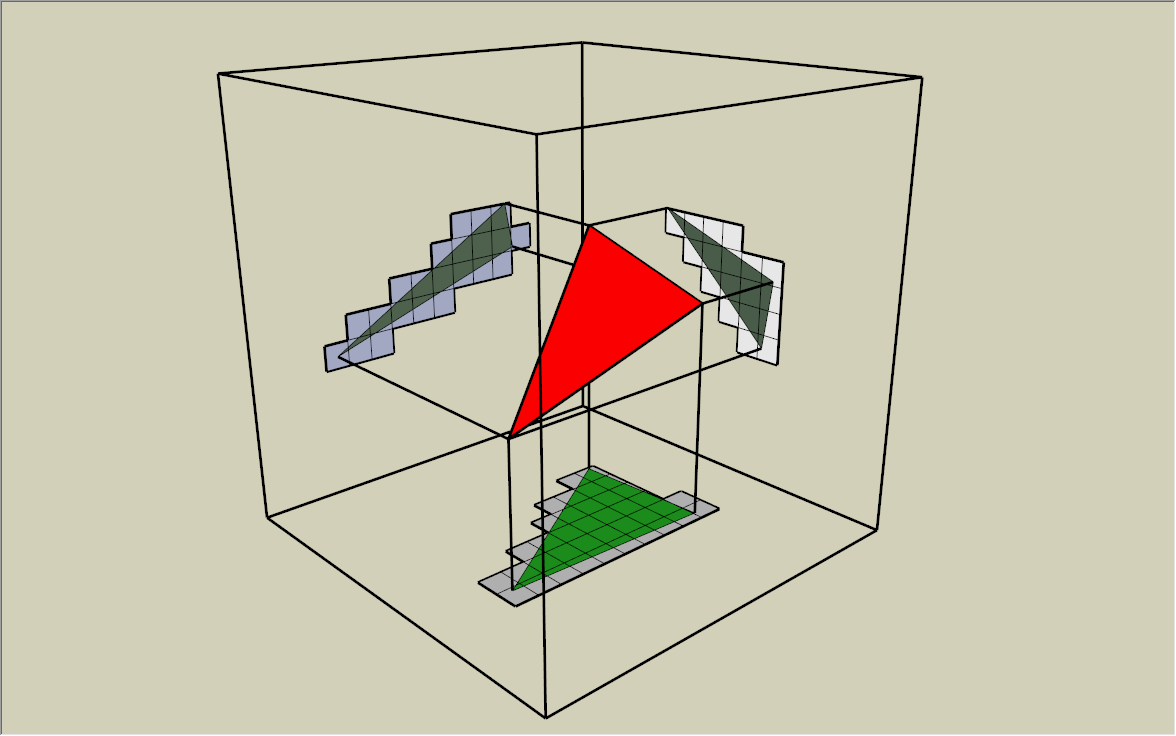
\includegraphics[width=\linewidth]{media/Voxelization_blog_fig_5.png}
		\caption*{Tres direcciones potenciales de proyección.}
	\end{subfigure}%
	\hspace{0.01\textwidth}
	\begin{subfigure}[t]{.49\linewidth}
		\centering
		\captionsetup{justification=centering}
		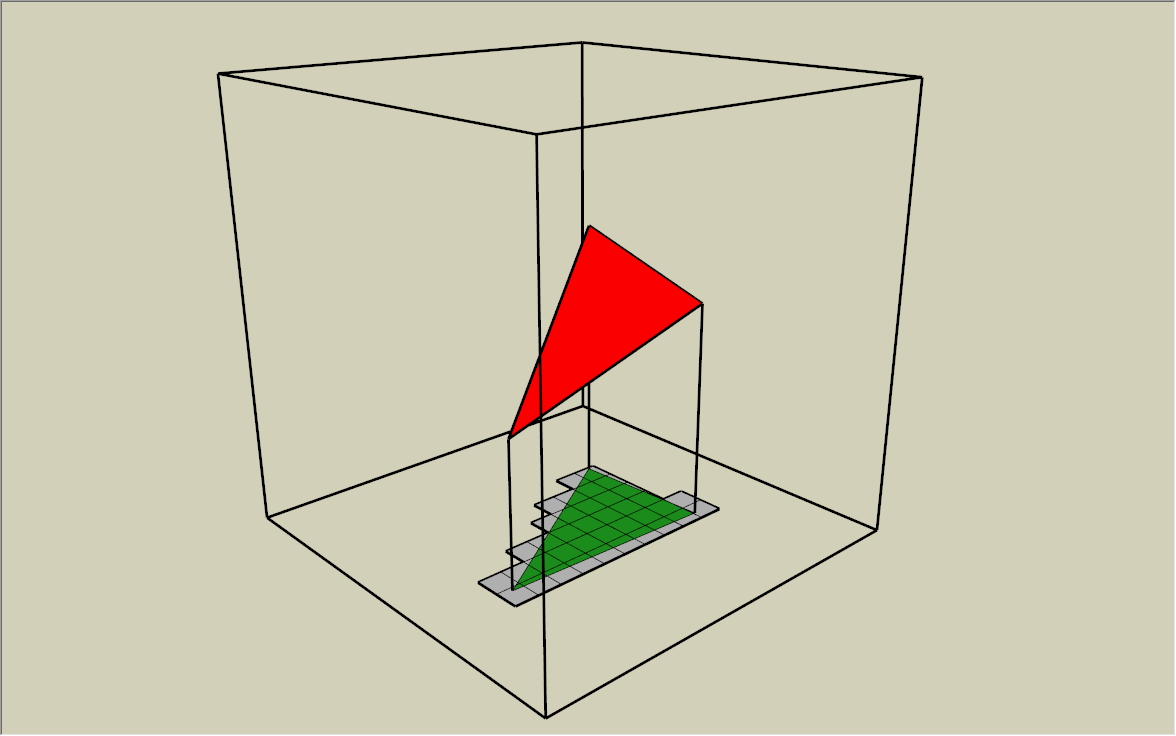
\includegraphics[width=\linewidth]{media/Voxelization_blog_fig_6.png}
		\caption*{Según el vector normal, proyección al eje Y es lo indicado.}
	\end{subfigure}%
	\caption{Descripción gráfica del proceso de selección del eje de proyección y maximización de fragmentos \cite{gpuvoxelization}.}
	\label{fig:axis_selection}
\end{figure}

\subsubsection{Extensión del Triángulo y Polígono Delimitante}
Una vez proyectados todos los vértices del triángulo según el eje direccional escogido (esto es multiplicar cada vértice por la matriz escogida) entonces se procede a expandir los vértices de este triángulo. Antes de esto primero es importante definir una \ac{AABB} para el triángulo. Esta area delimitante es utilizada en el \emph{fragment shader} para descartar fragmentos excedentes del triángulo expandido. El punto mínimo y máximo se expanden según la longitud diagonal de un píxel, en nuestra implementación este valor es $\frac{1}{V_{res}}$ donde $V_{res}$ representa la resolución del volumen. El Código \ref{AxisAlignedBoundingBox} expone como se genera este \ac{AABB}.  El arreglo \emph{pos} contiene los vértices del triángulo proyectado.
\\
\begin{lstlisting}[caption={Creación de un \ac{AABB} para el triángulo proyectado.}, label=AxisAlignedBoundingBox]
vec4 AxisAlignedBoundingBox(vec4 pos[3], vec2 pixelDiagonal)
{
    vec4 aabb;
    // punto mínimo y máximo para definir el aabb
    aabb.xy = min(pos[2].xy, min(pos[1].xy, pos[0].xy));
    aabb.zw = max(pos[2].xy, max(pos[1].xy, pos[0].xy));
    // se extiende el aabb por la longitud diagonal de un píxel
    aabb.xy -= pixelDiagonal;
    aabb.zw += pixelDiagonal;
    return aabb;
}
\end{lstlisting}

Luego en el Código \ref{TPlanes} primero se calculan los planos perpendiculares al triángulo formados por cada par de vértices del triángulo. Estos planos son trasladados medio píxel hacia afuera con respecto al triángulo proyectado.
\\
\begin{lstlisting}[caption={Planos por cada par de vértices del triángulo proyectado.}, label=TPlanes]
vec2 halfPixel = vec2(1.0f / volumeDimension);
// cálculo de planos perpendiculares al triángulo
vec3 planes[3];
planes[0] = cross(pos[0].xyw - pos[2].xyw, pos[2].xyw);
planes[1] = cross(pos[1].xyw - pos[0].xyw, pos[0].xyw);
planes[2] = cross(pos[2].xyw - pos[1].xyw, pos[1].xyw);
planes[0].z -= dot(halfPixel, abs(planes[0].xy));
planes[1].z -= dot(halfPixel, abs(planes[1].xy));
planes[2].z -= dot(halfPixel, abs(planes[2].xy));
\end{lstlisting}

Luego se calcula la intersección entre los planos perpendiculares al triángulo como se muestra en el Código \ref{TPlanes2}.
\\
\begin{lstlisting}[caption={Intersección entre planos perpendiculares al triángulo proyectado.}, label=TPlanes2]
// puntos de intersección entre los planos perpendiculares
vec3 intersection[3];
intersection[0] = cross(planes[0], planes[1]);
intersection[1] = cross(planes[1], planes[2]);
intersection[2] = cross(planes[2], planes[0]);
intersection[0] /= intersection[0].z;
intersection[1] /= intersection[1].z;
intersection[2] /= intersection[2].z;
\end{lstlisting}

En el Código \ref{TPlanes3} finalmente se obtienen los vértices del triángulo expandido al dilatar cada vértice según el plano del triángulo y los puntos de intersección.
\\
\begin{lstlisting}[caption={Vértices del triángulo expandido.}, label=TPlanes3]
vec4 trianglePlane;
// plano del triángulo proyectado en formato normal-distancia
trianglePlane.xyz = cross(pos[1].xyz - pos[0].xyz, pos[2].xyz - pos[0].xyz);
trianglePlane.xyz = normalize(trianglePlane.xyz);
trianglePlane.w = -dot(pos[0].xyz, trianglePlane.xyz);
// dilatación de los vértices del triángulo
float z[3];
z[0] = (-intersection[0].x * trianglePlane.x - intersection[0].y * trianglePlane.y - trianglePlane.w) / trianglePlane.z;
z[1] = (-intersection[1].x * trianglePlane.x - intersection[1].y * trianglePlane.y - trianglePlane.w) / trianglePlane.z;
z[2] = (-intersection[2].x * trianglePlane.x - intersection[2].y * trianglePlane.y - trianglePlane.w) / trianglePlane.z;
// posición final de los tres vértices del triángulo expandido
pos[0].xyz = vec3(intersection[0].xy, z[0]);
pos[1].xyz = vec3(intersection[1].xy, z[1]);
pos[2].xyz = vec3(intersection[2].xy, z[2]);
\end{lstlisting}

Este nuevo triángulo expandido es enviado al pipeline de rasterización donde cada fragmento generado será procesado por el \emph{fragment shader}. En el \emph{fragment shader} se almacenaran los datos de la escena sobre cada volumen de vóxeles.

\subsubsection{Composición de Fragmentos y Vóxeles}

Este proceso se realiza en el \emph{fragment shader}. En la sección anterior se mencionó la creación de una \ac{AABB} para el triángulo expandido. Lo primero a realizar durante la composición de fragmentos es descartar los fragmentos excedentes del triángulo:
\\
\begin{lstlisting}[caption={Descarte de fragmentos excedentes en el \emph{fragment shader}.}, label=TPlanes4]
// posición del fragmento debe encontrarse dentro del aabb
if( In.position.x < In.triangleAABB.x || In.position.y < In.triangleAABB.y || 
	In.position.x > In.triangleAABB.z || In.position.y > In.triangleAABB.w )
{
	discard;
}
\end{lstlisting}

En el Código \ref{TPlanes4} se compara la posición del fragmento con los límites del \ac{AABB}, si este se encuentra fuera de la \ac{AABB} del triángulo entones este fragmento es descartado. Esto resulta finalmente en un polígono delimitante ya descrito en la Figura \ref{fig:expanded_bbpolygon}.

Una vez ya finalizada la rasterización conservativa de cada triángulo, ahora se procede a almacenar la información de la escena en texturas tridimensionales. En nuestra aplicación se almacena en vóxeles el albedo, normal, y emisión de la geometría en escena. Un vóxel puede envolver a varios fragmentos y cada uno de estos fragmentos puede tener distintos valores para los atributos mencionados. Una forma simple de almacenar todos estos valores es utilizando un promedio de todos los valores por fragmento que envuelve el vóxel. 

Como se mencionó en la sección \ref{sub:frag_voxels}: cada fragmento es tratado como un hilo individual por tanto no hay forma de saber el orden como se envían fragmentos a la posición de un vóxel. La extensión \emph{GL\_ARB\_shader\_image\_load\_store} provee instrucciones atómicas para solventar esto. La forma más simple de obtener un promedio consistiria en utilizar la función \emph{imageAtomicAdd} y luego dividir por la cantidad de fragmentos. Para mantener un conteo de estos fragmentos se necesita un contador por cada vóxel. La idea es utilizar el canal alfa en un formato RGBA como contador. 

Sin embargo todas las funciones atómicas en esta extensión solo están reservadas para imágenes con formato entero de 32 bits. Generalmente el formato apropiado para estos valores seria RGBA8 o RGBA16F. Por tanto la función \emph{imageAdd} no puede ser utilizada para este propósito.

Se utiliza entonces la función \emph{atomicCompSwap} para emular la adición atómica. La idea es iterar por cada escritura sobre el volumen hasta que ya no haya más conflictos entre fragmentos y el valor actual del vóxel no ha sido cambiado por otro hilo de algún fragmento.

El promedio en cada vóxel debe ser calculado de forma incremental. Con el formato RGBA8 solo 8 bits están disponibles por canal. Por tanto es sencillo sobrepasar el valor límite de este formato mientras se suman valores. Para hacer esto se utiliza la siguiente fórmula:

\begin{equation}
	C_{i+1} = \frac{iC_{i}+x_i+1}{i+1}
\end{equation}

El Código \ref{imageAtomicRGBA8Avg} expone este procedimiento y la conversión entre formato RGBA8 y R32UI, sobre este último formato es posible realizar operaciones atómicas.
\\
\begin{lstlisting}[caption={Conversion entre RGBA8 y R32UI y promedio incremental.}, label=imageAtomicRGBA8Avg]
// conversion de formato de entero en r32ui a vec4
vec4 convRGBA8ToVec4(uint val)]
{
    return vec4(float((val & 0x000000FF)), 
    float((val & 0x0000FF00) >> 8U), 
    float((val & 0x00FF0000) >> 16U), 
    float((val & 0xFF000000) >> 24U));
}
// conversion de formato vec4 a entero r32ui
uint convVec4ToRGBA8(vec4 val)
{
    return (uint(val.w) & 0x000000FF) << 24U | 
    (uint(val.z) & 0x000000FF) << 16U | 
    (uint(val.y) & 0x000000FF) << 8U | 
    (uint(val.x) & 0x000000FF);
}
// promedio con atomicidad
void imageAtomicRGBA8Avg(layout(r32ui) volatile coherent uimage3D grid, ivec3 coords, vec4 value)
{
    // conversión de 0->1 a 0->255
    value.rgb *= 255.0;
    // valor equivalente en entero sin signo
    uint newVal = convVec4ToRGBA8(value);
    uint prevStoredVal = 0;
    uint curStoredVal;
    uint numIterations = 0;

    // mientras el valor almacenado sea diferente al actual y 
    // no se sobrepase el numero máximo de iteraciones
    while((curStoredVal = imageAtomicCompSwap(grid, coords, prevStoredVal, newVal)) 
            != prevStoredVal
            && numIterations < 255)
    {
        prevStoredVal = curStoredVal;
        vec4 rval = convRGBA8ToVec4(curStoredVal);
        rval.rgb = (rval.rgb * rval.a); // De-normalizar
        vec4 curValF = rval + value;    // Agregar nuevo valor
        curValF.rgb /= curValF.a;       // Re-normalizar
        newVal = convVec4ToRGBA8(curValF);
        ++numIterations;
    }
}
\end{lstlisting}

La función \emph{imageAtomicRGBA8Avg} es llamada por cada fragmento para almacenar el vector normal, el albedo y la emisión del promedio de todos los fragmentos sobre el espacio que envuelve un vóxel, estos vóxeles se almacenan en texturas tridimensionales como se muestra en el Código \ref{Voxelization2}.
\\
\begin{lstlisting}[caption={Composición de fragmentos y vóxeles}, label=Voxelization2]
// volúmenes utilizados para almacenar información de escena en vóxeles
layout(binding = 0, r32ui) uniform volatile coherent uimage3D voxelAlbedo;
layout(binding = 1, r32ui) uniform volatile coherent uimage3D voxelNormal;
layout(binding = 2, r32ui) uniform volatile coherent uimage3D voxelEmission;

void main()
{
(*@\centerline{\raisebox{-1pt}[0pt][0pt]{$\vdots$}}@*)
    // llamadas al promedio atómico por fragmento
    imageAtomicRGBA8Avg(voxelNormal, position, normal);
    imageAtomicRGBA8Avg(voxelAlbedo, position, albedo);
    imageAtomicRGBA8Avg(voxelEmission, position, emissive);
(*@\centerline{\raisebox{-1pt}[0pt][0pt]{$\vdots$}}@*)
}
\end{lstlisting}

\subsubsection{Bandera Estática}
El proceso de voxelización para geometría estática y dinámica es el mismo. Como se explicó en la sección \ref{sub:voxelizacion_dinamica} en nuestra implementación se evitó la creación de nuevos volúmenes para vóxeles estáticos y dinámicos. Para garantizar esto se utiliza un volumen con un solo componente entero, formato R8.

Durante la voxelización estática se almacena en este volumen un valor para marcar esta posición como estática (en este caso valor 1) como se observa en el Código \ref{Voxelization3}. 
\\
\begin{lstlisting}[caption={Escritura de la bandera estática durante voxelización de geometría estática}, label=Voxelization3]
layout(binding = 3, r8) uniform image3D staticVoxelFlag;

void main()
{
(*@\centerline{\raisebox{-1pt}[0pt][0pt]{$\vdots$}}@*)
    // durante voxelización estática se escribe la bandera sobre el volumen
    if(flagStaticVoxels)
    {
        imageStore(staticVoxelFlag, position, vec4(1.0));
    }
(*@\centerline{\raisebox{-1pt}[0pt][0pt]{$\vdots$}}@*)
}
\end{lstlisting}

En contraste durante la voxelización dinámica se lee este volumen para descartar la escritura sobre vóxeles estáticos como se observa en el Código \ref{Voxelization4}.
\\
\begin{lstlisting}[caption={Lectura de la bandera estática durante voxelización de geometría dinámica.}, label=Voxelization4]
(*@\centerline{\raisebox{-1pt}[0pt][0pt]{$\vdots$}}@*)
    // durante voxelización dinámica se lee la bandera sobre el volumen
    if(!flagStaticVoxels)
    {
        bool isStatic = imageLoad(staticVoxelFlag, position).r > 0.0f;
        // si la posición del vóxel es estática se descarta el fragmento cancelando la escritura
        if(isStatic) { discard; }
    }
(*@\centerline{\raisebox{-1pt}[0pt][0pt]{$\vdots$}}@*)
\end{lstlisting}

\subsection{Re-voxelización y Limpieza de Volúmenes}
Cada vez que se re-voxeliza la escena los volúmenes utilizados durante el proceso de voxelización deben ser limpiados antes de usarse. Para la voxelización estática esto es sencillo, OpenGL provee una función llamada \emph{glClearImage} desde la versión 4.4 la cual permite llenar una textura con un valor indicado. Debido a que se utiliza el mismo volumen para la voxelización dinámica no se puede utilizar esta función durante la voxelización dinámica ya que se eliminarían todos los vóxeles estáticos. Para solventar esto, antes de llamar al proceso de voxelización con la geometría dinámica se limpian del volumen todos los vóxeles que no son estáticos utilizando un \emph{compute shader}:
\\
\begin{lstlisting}[caption={Limpieza de vóxeles no estáticos.}, label=ClearVoxels]
void main()
{
    int volumeDimension = imageSize(voxelAlbedo).x;

    if(gl_GlobalInvocationID.x >= volumeDimension ||
        gl_GlobalInvocationID.y >= volumeDimension ||
        gl_GlobalInvocationID.z >= volumeDimension) return;

    ivec3 writePos = ivec3(gl_GlobalInvocationID);
    // vóxel vacío
    if(imageLoad(voxelAlbedo, writePos).a < EPSILON) { return; }
    // vóxel es estático
    if(texelFetch(staticVoxelFlag, writePos, 0).r > EPSILON) { return; }
    // vóxel no es estático entonces se procede a limpiar el volumen con ceros
    imageStore(voxelAlbedo, writePos, vec4(0.0));
    imageStore(voxelNormal, writePos, vec4(0.0));
    imageStore(voxelEmissive, writePos, vec4(0.0));
}
\end{lstlisting}

En el Código \ref{ClearVoxels} primero se verifica si ya el vóxel está vacío, luego si este es estático y finalmente si este no lo es se le coloca el valor cero en todos los canales de color y el alfa, esto indica que allí no hay un vóxel.
% section pipeline_de_voxelizacion (end)
